% 
% Kringverkiezing
% @author Pieter Maene <pieter.maene@student.kuleuven.be>
%

%TODO Analyse

\chapter{Kringverkiezing}
\label{chap:kringverkiezing}

Het Helios verkiezingssysteem werd in de praktijk gebruikt tijdens de kringverkiezing van de Vlaamse Technische Kring. Dit is de faculteitskring van de studenten burgerlijk ingenieur aan de KU Leuven. Om het systeem hiervoor te kunnen gebruiken, waren enkele aanpassingen nodig die overlopen worden in \ref{sec:kv:aanpassingen}. Gezien het cruciale karakter van een verkiezing, werd het systeem vervolgens uitgebreid getest (\ref{sec:kv:testen}). Tot slot wordt het verloop van de stemdag zelf besproken in \ref{sec:kv:stemdag}.

\section{Aanpassingen}
\label{sec:kv:aanpassingen}

\subsection{Shibboleth}

Shibboleth is het authenticatie mechanisme dat gebruikt wordt voor de centrale login van de KU Leuven. Iedere gebruiker kan uniek ge\"identificeerd worden aan de hand van zijn studentennummer. Alle stemgerechtigde kiezers voor een kringverkiezing hebben een dergelijke account. Helios had hier echter nog geen ondersteuning voor. Gezien het modulaire ontwerp van het authenticatiesysteem, was dit relatief eenvoudig toe te voegen.

\npar De kieslijsten zelf werden opgemaakt door LOKO, de Leuvense studentenkoepel. Deze moesten wel nog omgezet worden naar een bestand dat uitgelezen kon worden door Helios. Het studentennummer werd hierbij gebruikt als het unieke ID voor elke kiezer. Een probleem was hier wel dat de e-mailadressen van de kiezers niet mee opgenomen waren in deze lijsten. Deze kunnen wel mee doorgegeven worden met het antwoord dat de server ontvangt nadat de student zich aangemeld heeft via de centrale login.

\subsection{Opkomst}

Bij VTK vertegenwoordigt het praesidium de studenten ook op onderwijsvlak. Om dit te kunnen doen, moet er volgens het reglement van LOKO een meerderheid behaald worden bij een opkomst van minstens 10\%.\cite{loko_kiesreglement_verkiezingen} De berekening van dit percentage werd dan ook toegevoegd zodat dit samen met de resultaten bekend gemaakt kon worden.

\subsection{Publicatie van het resultaat}

Helios publiceert het resultaat van de verkiezing standaard van zodra het bekend is. Het is echter traditie om deze pas om middernacht bekend te maken. Het systeem moest hier dus licht voor aangepast worden.

\section{Testen}
\label{sec:kv:testen}

Om er zeker van te zijn dat het systeem op de stemdag zelf goed zou functioneren, werd het na de installatie op de server getest. Hierbij werd niet alleen nagegaan of alles technisch in orde was, maar werd ook feedback gevraagd over de gebruiksvriendelijkheid. 

\npar De testen van het beheer (\ref{sec:kv:beheer}) en het stemhokje (\ref{sec:kv:stemhokje}) werden uitgevoerd in de context van de verkiezingen bij VTK, die hier wat verder belicht wordt. Het Neutraal Comit\'e, dat alles in goede banen leidt, wordt bij VTK aangeduid met VKK. De huidige praeses is hier steeds de voorzitter van. Hij wordt geholpen door een aantal vrijwilligers uit het praesidium die geen kandidaat zijn. Er zijn twee verschillende types kiesploegen bij VTK. Enerzijds zijn er de serieuze ploegen die opkomen als praesidium voor het volgende jaar en anderzijds de lolploegen die niet als vertegenwoordigers verkiesbaar zijn.

\subsection{Beheer}
\label{sec:kv:beheer}

Aangezien hier de meeste veranderingen gebeurd zijn (\ref{sec:ui:beheer}), moest zeker dit deel goed getest worden. Hiervoor werd een testverkiezing aangemaakt door de voorzitter van VKK, met de echte trustees en vragen. De echte kieslijsten werden vervangen door een lijst met de huidige praesidiumleden.

\npar De trustees voor de verkiezing zijn de zes leden van VKK. Als threshold schema (\ref{sec:helios:threshold_encryptie}) werd ervoor gekozen dat drie van hen nodig zijn om het resultaat te decrypteren. Tijdens deze test kwamen echter twee fouten naar boven. Ten eerste werd de Lagrange-interpolatie niet over het eindig veld berekend, maar met een rationale breuk. Wanneer slechts twee trustees gebruikt werden, was dit geen probleem omdat de noemer dan gelijk is aan \'e\'en. Dit kon eenvoudig opgelost worden door de teller en noemer voor het hele product apart te berekenen (\ref{eq:kv:modular_lagrange_numerator} en \ref{eq:kv:modular_lagrange_denominator}). Vervolgens wordt de teller vermenigvuldigd met de modulaire inverse van de noemer (\ref{eq:kv:modular_lagrange_result}).

\begin{align}
  \label{eq:kv:modular_lagrange_numerator} 
  N_i & = \prod_{j=1, j\not=i}^k{-x_j} \mod{q} \\
  \label{eq:kv:modular_lagrange_denominator}
  D_i & = \prod_{j=1, j\not=i}^k{(x_i - x_j)} \mod{q} \\
  \label{eq:kv:modular_lagrange_result}
  \lambda{_i}(0) & = N_i * (D_i^{-1} \mod{q}) \mod{q}
\end{align}

\npar Ten tweede werd de Helios trustee automatisch toegevoegd als trustee aan de verkiezing. Alle acties die een trustee moet uitvoeren, waren hiervoor geautomatiseerd. Na het uitvoeren van een aantal tests bleek dat de shares van deze trustee niet compatibel waren met deze van de anderen. Het grote verschil tussen beide is dat deze van Helios in Python en niet in JavaScript gegenereerd werden. Omdat er niet direct een fout gevonden kon worden, werd ervoor gekozen om Helios niet langer als trustee toe te voegen. Omdat alles hiervoor geautomatiseerd was, had deze toch niet zo'n belangrijke rol binnen het proces. Hij werd voornamelijk toegevoegd omdat dan een verkiezing zonder eigen trustees opgezet kon worden, wat leidt tot een eenvoudigere procedure.

\npar Verder verliep deze test zeer goed. De voorzitter kon zonder hulp de volledige procedure (\ref{chap:procedure}) voor het aanmaken van een verkiezing met threshold encryptie doorlopen. Er werd verder geen formele analyse van de nieuwe interface gemaakt, aangezien deze slechts door een beperkt aantal mensen gebruikt zal worden. Ook de trustees hadden weinig moeite om hun geheime sleutels te bekomen. Ondanks de e-mails die verstuurd worden telkens een actie van hen nodig is, duurde het nog steeds even voordat dit in orde was.

\subsection{Stemhokje}
\label{sec:kv:stemhokje}

Tijdens het testen kwamen geen functionele problemen naar voor met het stemhokje. Toch kwam ook hier veel feedback op van het praesidium. Veel mensen vonden het stemmen niet intu\"itief. Er waren twee belangrijke bemerkingen. Ten eerste waren sommige bewoordingen te ingewikkeld. De interface is volledig in het Engels en er kwamen veel onbekende vaktermen in voor. Dit kon eenvoudig opgelost worden door eenvoudigere terminologie in de plaats te gebruiken.

\npar Ten tweede vonden velen het proces te moeilijk. Oorspronkelijk waren er vier stappen. Gebruikers kregen eerst een korte uitleg, gevolgd door het aanduiden van hun keuzes. Hierna konden deze gecontroleerd worden, waarna de stem ge\"encrypteerd werd. Daarna volgde nog een scherm (\ref{fig:kv:booth_submit}) waar gekozen kon worden om een audit te doen van de stem of ze te uploaden. In het laatste geval werd het stemhokje verlaten, maar moest de gebruiker nog eens bevestigen dat hij zijn stem wilde uitbrengen. Vooral deze twee laatste stappen vonden veel mensen verwarrend.

\begin{figure}
  \center{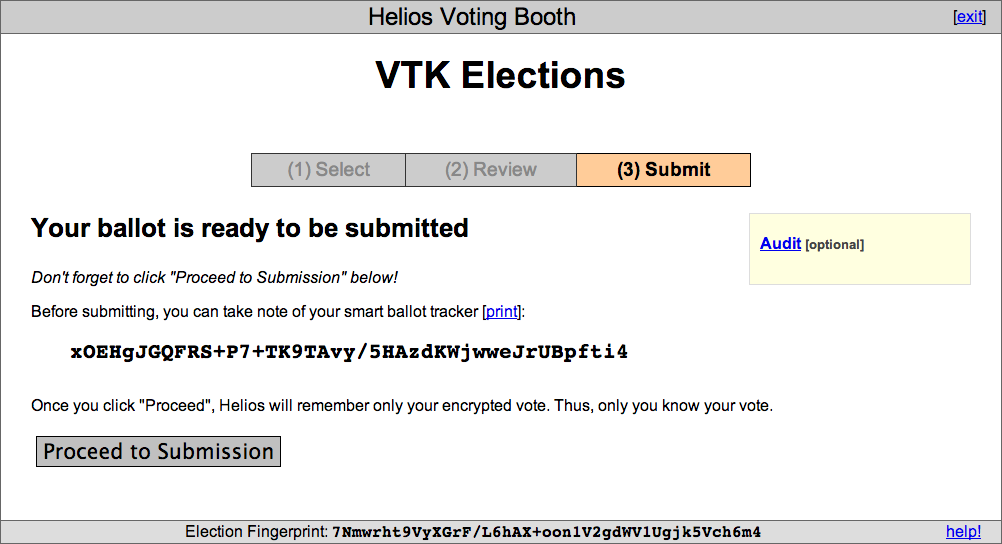
\includegraphics[width=\linewidth]{kv/booth_submit.png}}
  \caption{Laatste scherm van het stemhokje}
  \label{fig:kv:booth_submit}
\end{figure}

\npar Om dit proces te vereenvoudigen, werd de laatste stap van het stemhokje verwijderd. Na het bevestigen van zijn keuzes, wordt de kiezer onmiddellijk doorgestuurd naar het uploaden buiten het stemhokje. De audit van een stem werd verplaatst naar het scherm waar de keuzes bevestigd moet worden. Omdat de stem hiervoor reeds ge\"encrypteerd moet zijn, wordt dit nu gedaan na het beantwoorden van de laatste vraag. Het grootste nadeel hierbij is dat de encryptie opnieuw uitgevoerd moet worden wanneer de kiezer zijn stem wijzigt. In de huidige implementatie gaat dit echter al relatief vlot in moderne browsers. In de toekomst zal dit waarschijnlijk nog sneller kunnen door gebruik te maken van de Web Cryptography API (\ref{chap:web_cryptography_api}).

\npar Na het aanpassen van het stemhokje werd deze test herhaald om zeker te zijn dat alles nog correct werkte. Ook tijdens deze test kwamen nog vragen om enkele kleine dingen te wijzigen voor de echte verkiezing. Zo wordt er een waarschuwing gegeven wanneer de kiezer het laatste scherm sluit voordat hij zijn stem ge\"upload heeft.

\begin{figure}
  \center{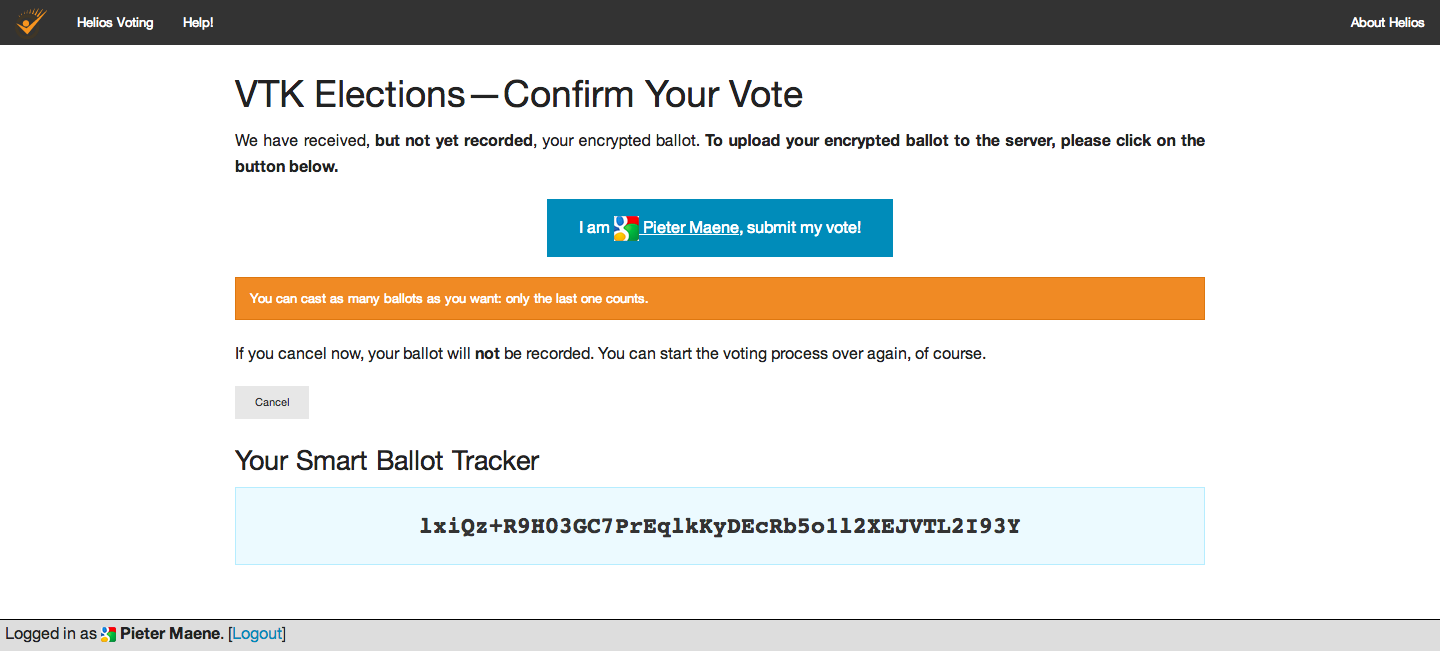
\includegraphics[width=\linewidth]{kv/cast_confirm.png}}
  \caption{Bevestigen van de stem}
  \label{fig:kv:cast_confirm}
\end{figure}

\subsection{Stresstest}

Er is elk jaar een opkomst van ongeveer 25\% bij de kringverkiezing van VTK, wat iets minder dan \np{1000} kiezers zijn. Daarom werd nagegaan of Helios ook een groot aantal stemmen nog correct kon verwerken. Hiervoor werd een aparte verkiezing aangemaakt met twee trustees en drie vragen. Vervolgens werden \np{1000} stemmen uitgebracht. Het resultaat kon van de eerste keer correct gedecrypteerd worden, dus hier was geen verdere actie nodig.

\npar Deze stemmen werden gegenereerd door een server-side actie. De kiezers stemmen normaal via het stemhokje, maar dat proces is moeilijk te automatiseren. Het grote verschil is dat de encryptie in Python in plaats van JavaScript gebeurt.

%TODO Remove Color

\npar \textcolor{red}{Deze test werd niet op de server maar lokaal uitgevoerd. Het doel was hierbij te kijken of decryptie ook bij een groot aantal stemmen correct functioneerde. De belasting op de server van een groot aantal kiezers werd niet onderzocht omdat iedere kiezer slechts een beperkt aantal lichte requests uivoert.}

\section{Stemdag}
\label{sec:kv:stemdag}

De stemming zelf vond plaats op donderdag 8 mei 2014. Oorspronkelijk stond ze open van 7u00 tot 19u00. Omdat de communicatie 's ochtends traag op gang gekomen was, werd dit verlengd tot 20u00, wat ondersteund wordt door Helios. De trustees en het threshold schema waren dezelfde als tijdens de test (\ref{sec:kv:beheer}). De vragen en het resultaat worden getoond in \ref{fig:kv:result}. In totaal hebben 768 mensen hun stem uitgebracht, wat niet significant minder is dan in andere jaren. Dit is dus een sterke indicatie dat het proces voldoende eenvoudig is. Zowel bij het stemmen als het decrypteren van het resultaat waren er geen problemen.

\begin{figure}
  \center{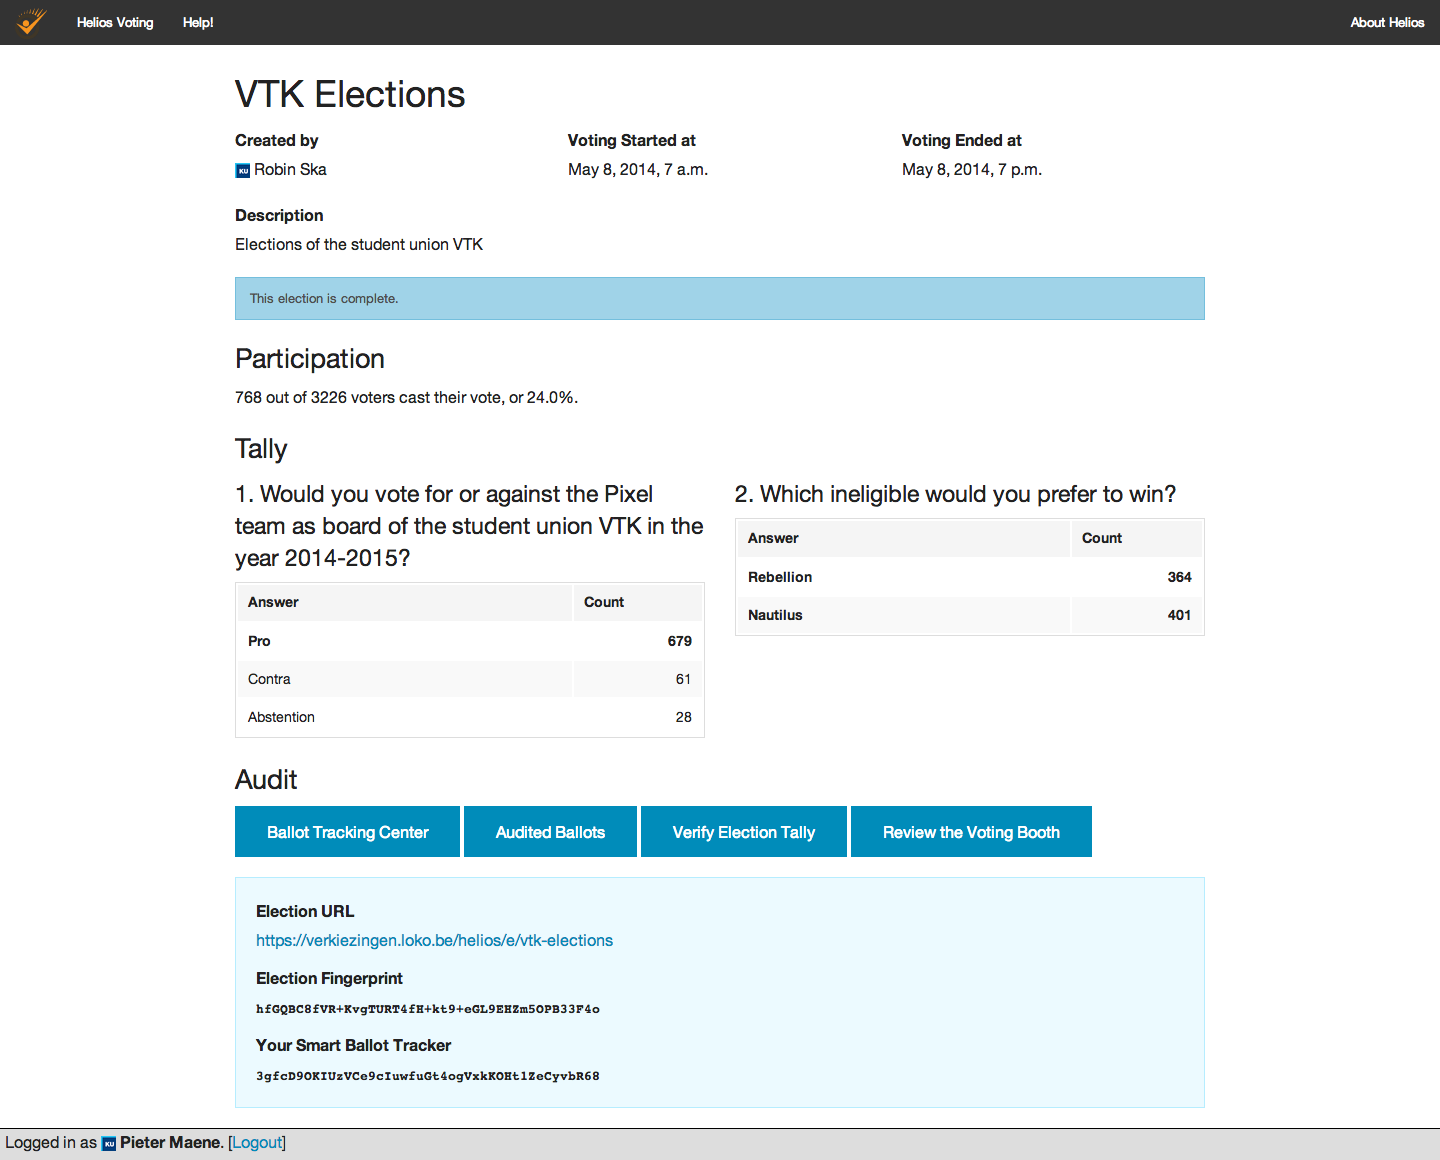
\includegraphics[width=\linewidth]{kv/result.png}}
  \caption{Resultaat van de stemming}
  \label{fig:kv:result}
\end{figure}
